\chapter{A search for new physics in events with a Z boson, missing transverse energy, and jets}

\section{Motivations}

This is some great motivation!

\subsection{Motivating Models} \label{sec:susy_models}

\begin{figure}[h!]
  \centering
  
\includegraphics[width=.5\textwidth]{figures/placeholder.png}
  \caption{\todo{To Be Updated Strong and EWK SUSY diagrams.}}
  \label{fig:SUSY-diagrams}
\end{figure}

1. Show the models Strong and EWK SUSY model diagrams we use here.
2. Discuss why they are useful tools (i.e. give an idea of SMS)

\section{Analysis Strategy}

\subsection{Background Considerations}

\subsubsection{Leptonic Final States} \label{sec:leptonic_final_states}
The Z boson can decay to any fermion. In theory, one could perform this analysis in an all hadronic final state, which might seem advantageous as the Z will decay to hadrons approximately 10 times as often as it will decay to light leptons. \todo{Add some figure for the Z decay rates, probably can site the PDG}. However, there are several reasons leptonic final states are highly advantageous.

In hadron colliders, the most common types of final states are those with only hadronic activity, as can be seen in figure \ref{fig:lhc_decay_modes}; leptonic final states provide a much cleaner population in which to search for Z bosons. Additionally, as referenced in \ref{sec:electron_measurement_pipeline}, \ref{sec:muon_measurement_pipeline}, and \ref{sec:MET_reco}, the fidelity of energy measurements for the light leptons is much better than for jets at CMS. This provides great advantage for background discrimination; leptons from Z boson decays will tend to have a very specific dilepton mass, a quantity reconstructed from the momentum measurements.

The decays of the Z produce two opposite sign, same flavor fermions. A further benefit of the leptonic channel is that flavor and charge identification is fairly easy for the light leptons but nearly impossible to identify for jets at the current state of the art (for instance, one can not say with high confidence that a jet was produced by a positively charged charm quark). Finally, the energy and momentum measurements for the light leptons are much better than for jets because of the complexity involved in making good energy measurements for jets. \todo{Point to some discussion about hadron calorimetry, the basic idea here is just that jets have neutral particles and their contribution to the energy measurement needs to be implied by the reconstruction algorithm} 

Therefore, even though the decay rate to light leptons from Z bosons is lower than the production rate to hadronic final states, the better energy resolution and lower background rate makes the leptonic final state far more powerful.

When using the leptonic final states, there are essentially two other background sources of leptons we must consider, these are $\gamma$ and W decays. The W boson will decay into leptons only with a complimentary neutrino, this means that in order to select a pair of opposite charge and same flavor leptons, there must be at least two W bosons in the event. Because the decays of the W will be independent, there is only a 50\% chance that the two leptons in an event where two Ws decay leptonically will have the same flavor. As will be discussed later, this makes the background prediction for these types of events very easy as events with two same flavor leptons can be used to model essentially any kinematical distribution.

Depending on the source of the Ws, the kinematics of the leptons will differ. However, a general rule is that the total energy in the event will be peaked at some low value, near the threshold to produce the event, essentially the sum of the mass of all the prompt particles, and decay exponentially from there. Many kinematic distributions are highly correlated with the total energy in the event. In the case of the Z decay, we know the dilepton mass distribution will not be correlated

It turns out the most common source of W bosons is through the production of two top quarks, which decay to a bottom quark and a W Boson. To reject these events, we will use B-tagging, described in \todo{add reference to b-tagging section}. Further, the dilepton mass in these events will be essentially random \todo{Add a figure of WW and TTBar production MLL plot for ZMET. Is the distribution flat or falling?} but biased towards lower values. 

less likely, whereas for Z decay, the breit-wigner distribution predisposes the dilepton mass to be near 91 GeV. 

The overall dilepton mass distribution will be a falling distribution with a small bump for the Z Boson. 

\todo{Need to close this off with a discussion about how the backgrounds are mainly DY, TTBar, and VZ}

Finally, due to the instability of the $\tau$ lepton, we neglect this channel from the search. $\tau$ leptons are much harder to identify than the light leptons, and further they can decay to light leptons in a flavor symmetric manner, so are predicted by that background channel's prediction method.

\subsubsection{Hadronic Activity Requirements}
As mentioned above, the major production mode of opposite sign dilepton pairs with dilepton mass near 91 GeV is from Drell-Yan production of Z. The diagram for this type of process is shown in \ref{fig:DY-diagram}. As can be seen in the figure, the leading order diagram for this process has no free quarks or gluons. That there are no free colored particles means that the vast majority of these events will likewise come without any jets. Diagrams with ISR and FSR which take a cross-section production hit of roughly 1/5 \todo{explain this}, which means that we can suppress the DY background by a factor of 100 by requiring at least 2 jets in an event. This keeps our signal count low. Further, the prediction of 0 or 1 jet bins is a completely different process due to the sources of MET, and many of our motivating models will have many jets as part of their decay chain. 

\begin{figure}[h!]
  \centering
  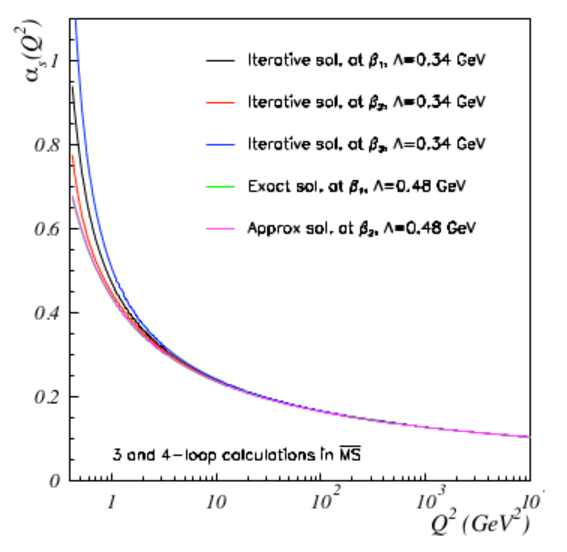
\includegraphics[width=.5\textwidth]{figures/QCD_Coupling_Running.pdf}
  \caption{The QCD coupling constant computed to different orders and different cutoff scales. The production of the Z boson is much more likely at center of mass energy near the mass of the Z. This means that $\alpha_s$ is between $\frac{1}{5}$ and $\frac{1}{10}$, which can be viewed as the zeroth order multiplicative correction to the DY with a single ISR or FSR jet cross section} 
  \label{fig:alpha_s_running}
\end{figure}

In fact, strongly produced SUSY models described in \ref{sec:susy_models} anticipate lots of hadronic activity. Therefore, in search regions targeted at those models, we also also ask for lots of hadronic activity by selecting events with high $H_T$, the scalar sum of transverse energy for all jets in an event, above certain thresholds. This further rejects DY events.

\begin{figure}[h!]
  \centering
  
\includegraphics[width=.5\textwidth]{figures/placeholder.png}
  \caption{\todo{To Be Updated with DY figure.}}
  \label{fig:DY-diagram}
\end{figure}

\subsection{MET Binning}
Again, inspecting the diagram above, when the Z decays to charged leptons, no neutrinos are produced. This means that DY has no genuine MET, any missing energy must come from mismeasurements of the jet energy, misattributions of jets to the DY vertex, or loss of objects out of the detectors fiducial area. These should be relatively small effects and we will discuss how we predict the MET distribution for this type of event in the following sections. For now, consider that the leading background when searching for Z bosons can be reduced dramatically by considering only events with high MET. In this analysis, we only look at events with more than 100 GeV of missing energy.

\subsection{MT2}
The MT2 variable is defined as

\[
\min\max{whatever}
\]

When a pair of W bosons decay into a lepton and a neutrino, we can see that this value should not be able to be larger than the mass of the W boson, since by summing over all possibilities, we will get the true values which makes the outer minimum select at most the mass of the W (there is no lower limit). However, in the case of an arbitrary decay, for instance in DY or in signal models with dark matter, there is no need for this value to be smaller than the mass of the W and generally higher values will be found. Therefore, we can use this quantity as a handle for rejecting events where the leptons come from two W bosons. We require in our signal regions that MT2 be at least greater than 80 GeV, near the mass of the W boson. This mainly rejects the TTBar background. \todo{Why does any TTBar actually get through?}

\subsection{B-Tagging}
We also like to bin in b-tags. This is because the background composition changes dramatically with b-tagging as the second largest background is TTBar. This allows us to use a slightly higher MT2 cut in regions with a b-tag, as they will be more dominated by TTBar than by DY since DY is likely not going to have a b-tag even though it might.

\section{Object And Event Selection}

  The selection of events can be broken into several stages. Preselection is essentially how we get our population of dilepton lepton events. As described in \ref{sec:datasets}, we seed all events through the CMS dilepton datasets. There are essentially 3 separate regions we select from. For the signal regions, we select events with dilepton pairs, for the falvor-symmetric background prediction, we select events with same sign dilepton pairs, for the MET templates prediction, we select from single photon events which are seeded by an entirely different dataset.

  This leaves us with events that have at least 2 lepton candidates above some nominal $p_T$ thresholds. The events are then refined further as described below.
  
  \subsection{Lepton Selection}
    For the signal selection, we require that our events have at least 2 opposite-charge same-flavor light leptons as identified by the CMS particle flow algorithm described in \rec{sec:particle_flow}. This means we have either $e^+e^-$ or $\mu^+ \mu^-$ pairs in each event. To predict the flavor symmetric background, we also use events with same-sign dilepton pairs. Additionally, we select events with no leptons and only

    \begin{itemize}
      \item The (sub)leading lepton in each event must have at least (20) 25 GeV of transverse momentum. These points were selected so that the event would be in the "trigger turn-on" described in \ref{sec:event_triggering}.
      \item The pseudorapidity for each lepton must be within the inner tracker's fiducial area, namely $\left|\eta\right| < 2.4$
      \item 
    \end{itemize}

    \subsubsection{Electron ID and Isolation}
    Transcribe ID and Iso requirements.

    \subsubsection{Muon ID and Isolation}

  \subsection{Jet Selection}

  \subsection{Photon Selection}

  \subsection{Isolated Tracks}

  \subsection{Search Regions}
    Electroweak search regions and strong search regions

\section{Background Estimation Methods}
Fakes are taken care of by the flavor symmetric BG.

\section{Results}

\section{Signal Interpretations} 

\section{The Electroweak Combination}

The things we want to consider here are: 

  1. All the cuts and stuff, I want to list out what cuts we made and why we chose them. I am not sure where I will put all the data/MC agreement stuff. I guess that's mostly important for the MET profile as I don't really use MC in the rest of the
